% -*- Mode:TeX -*-

%% The documentclass options along with the pagestyle can be used to generate
%% a technical report, a draft copy, or a regular thesis.  You may need to
%% re-specify the pagestyle after you \include  cover.tex.  For more
%% information, see the first few lines of mitthesis.cls. 

%\documentclass[12pt,vi,twoside]{mitthesis}
%%
%%  If you want your thesis copyright to you instead of MIT, use the
%%  ``vi'' option, as above.
%%
%\documentclass[12pt,twoside,leftblank]{mitthesis}
%%
%% If you want blank pages before new chapters to be labelled ``This
%% Page Intentionally Left Blank'', use the ``leftblank'' option, as
%% above. 

\documentclass[12pt,twoside]{mitthesis}
\usepackage{lgrind}
\usepackage{graphicx}
\usepackage{url}
\pagestyle{plain}

%% This bit allows you to either specify only the files which you wish to
%% process, or `all' to process all files which you \include.
%% Krishna Sethuraman (1990).

\typein [\files]{Enter file names to process, (chap1,chap2 ...), or `all' to
process all files:}
\def\all{all}
\ifx\files\all \typeout{Including all files.} \else \typeout{Including only \files.} \includeonly{\files} \fi

\begin{document}

%% define some macros here
\newcommand{\cphash}{{\sc CPHash}}
\newcommand{\cpserver}{{\sc CPServer}}
\newcommand{\lockhash}{{\sc LockHash}}
\newcommand{\lockserver}{{\sc LockServer}}
\newcommand{\memcached}{{\sc Memcached}}

% -*-latex-*-

% NOTE:
% These templates make an effort to conform to the MIT Thesis specifications,
% however the specifications can change.  We recommend that you verify the
% layout of your title page with your thesis advisor and/or the MIT 
% Libraries before printing your final copy.
\title{\cphash: A Cache-Partitioned Hash Table with LRU Eviction}

\author{Zviad Metreveli}
% If you wish to list your previous degrees on the cover page, use the 
% previous degrees command:
%       \prevdegrees{A.A., Harvard University (1985)}
% You can use the \\ command to list multiple previous degrees
%       \prevdegrees{B.S., University of California (1978) \\
%                    S.M., Massachusetts Institute of Technology (1981)}
\department{Department of Electrical Engineering and Computer Science}

% If the thesis is for two degrees simultaneously, list them both
% separated by \and like this:
% \degree{Doctor of Philosophy \and Master of Science}
\degree{Master of Engineering in Electrical Engineering and Computer Science}

% As of the 2007-08 academic year, valid degree months are September, 
% February, or June.  The default is June.
\degreemonth{June}
\degreeyear{2011}
\thesisdate{May 18, 2011}

%% By default, the thesis will be copyrighted to MIT.  If you need to copyright
%% the thesis to yourself, just specify the `vi' documentclass option.  If for
%% some reason you want to exactly specify the copyright notice text, you can
%% use the \copyrightnoticetext command.  
%\copyrightnoticetext{\copyright IBM, 1990.  Do not open till Xmas.}

% If there is more than one supervisor, use the \supervisor command
% once for each.
\supervisor{M. Frans Kaashoek}{Professor}
\supervisor{Nickolai Zeldovich}{Assistant Professor}

% This is the department committee chairman, not the thesis committee
% chairman.  You should replace this with your Department's Committee
% Chairman.
\chairman{Dr. Christopher J. Terman}{Chairman, Department Committee on Graduate Theses}

% Make the titlepage based on the above information.  If you need
% something special and can't use the standard form, you can specify
% the exact text of the titlepage yourself.  Put it in a titlepage
% environment and leave blank lines where you want vertical space.
% The spaces will be adjusted to fill the entire page.  The dotted
% lines for the signatures are made with the \signature command.
\maketitle

% The abstractpage environment sets up everything on the page except
% the text itself.  The title and other header material are put at the
% top of the page, and the supervisors are listed at the bottom.  A
% new page is begun both before and after.  Of course, an abstract may
% be more than one page itself.  If you need more control over the
% format of the page, you can use the abstract environment, which puts
% the word "Abstract" at the beginning and single spaces its text.

%% You can either \input (*not* \include) your abstract file, or you can put
%% the text of the abstract directly between the \begin{abstractpage} and
%% \end{abstractpage} commands.

% First copy: start a new page, and save the page number.
\cleardoublepage
% Uncomment the next line if you do NOT want a page number on your
% abstract and acknowledgments pages.
% \pagestyle{empty}
\setcounter{savepage}{\thepage}
\begin{abstractpage}
%% The text of your abstract and nothing else (other than comments) goes here.
%% It will be single-spaced and the rest of the text that is supposed to go on
%% the abstract page will be generated by the abstractpage environment.  This
%% file should be \input (not \include 'd) from cover.tex.

In this thesis we introduce \cphash{} $-$ a scalable fixed size hash table that supports eviction
using an LRU list, and \cpserver{} $-$ a scalable in memory key/value cache server that uses \cphash{} 
to implement its hash table. \cphash{} uses computation migration to avoid transferring data between cores. 
Experiments on a 48 core machine show that \cphash{} has 2 to 3 times higher throughput than a hash
table implemented using scalable fine-grained locks. \cpserver{} achieves
1.2 to 1.7 times higher throughput than a key/value cache server that uses a hash table with
scalable fine-grained locks and 1.5 to 2.6 times higher throughput than \memcached{}.

\end{abstractpage}

% Additional copy: start a new page, and reset the page number.  This way,
% the second copy of the abstract is not counted as separate pages.
% Uncomment the next 6 lines if you need two copies of the abstract
% page.
% \setcounter{page}{\thesavepage}
% \begin{abstractpage}
% %% The text of your abstract and nothing else (other than comments) goes here.
%% It will be single-spaced and the rest of the text that is supposed to go on
%% the abstract page will be generated by the abstractpage environment.  This
%% file should be \input (not \include 'd) from cover.tex.

In this thesis we introduce \cphash{} $-$ a scalable fixed size hash table that supports eviction
using an LRU list, and \cpserver{} $-$ a scalable in memory key/value cache server that uses \cphash{} 
to implement its hash table. \cphash{} uses computation migration to avoid transferring data between cores. 
Experiments on a 48 core machine show that \cphash{} has 2 to 3 times higher throughput than a hash
table implemented using scalable fine-grained locks. \cpserver{} achieves
1.2 to 1.7 times higher throughput than a key/value cache server that uses a hash table with
scalable fine-grained locks and 1.5 to 2.6 times higher throughput than \memcached{}.

% \end{abstractpage}

\cleardoublepage

\section*{Acknowledgments}

Foremost, I would like to thank my advisors, Frans Kaashoek and Nickolai Zeldovich, for all their help and guidance during this project. 
I've learned a lot while working with them this year.

I would also like to thank MIT for giving me an opportunity to be a part of its truly inspiring community.

Thank you to my girlfriend for being there for me and all her help and care.

Finally, I would like to thank my family. I would like to thank my brother for his friendship and support throughout 
the years and my parents for always encouraging me to follow my aspirations.

%%%%%%%%%%%%%%%%%%%%%%%%%%%%%%%%%%%%%%%%%%%%%%%%%%%%%%%%%%%%%%%%%%%%%%
% -*-latex-*-

\pagestyle{plain}
  % -*- Mode:TeX -*-
%% This file simply contains the commands that actually generate the table of
%% contents and lists of figures and tables.  You can omit any or all of
%% these files by simply taking out the appropriate command.  For more
%% information on these files, see appendix C.3.3 of the LaTeX manual. 
\tableofcontents
%%\newpage
%%\listoffigures
%%\newpage
%%\listoftables


\chapter{Introduction}
\label{chap:intro}

Hash tables are heavily used data structures in distributed data centers and web servers. This thesis focuses
on fixed-size hash tables that support eviction of its elements using a Least Recently Used (LRU) list. Such hash tables are a good way to
implement a key/value cache. One of the best known distributed applications that uses a key/value cache is 
\memcached{} \cite{memcached}. \memcached{} is an in-memory cache for Web applications that store  
data, page rendering results, and other information that can be cached and is expensive to recalculate.

With the rapid growth of the World Wide Web and large-scale applications, more scalability is demanded from data structures. 
Although many data structures and applications are already developed with the scalability requirement in mind, 
they are usually designed for distributed systems that consist of multiple different machines. The recent emergence of multi-core 
architectures demands that we rethink scalability not just for scaling across multiple machines but also across 
multiple cores of the same machine. 

This thesis explores the use of \textit{computation migration} to increase data structure performance on 
multi-core processors. This technique can also be applied to structures other than the hash table. We chose the 
hash table to demonstrate the benefits of this idea because of its overall simplicity, ease of implementation and relevance.

\section{Motivation}

Since CPU frequencies can no longer be significantly increased due to heat and power dissipation challenges, 
processors are now becoming more powerful by having more and more separate computation cores. Thus, if we want to 
get better performance as the number of cores increases, we need to think of ways to make our applications more scalable across 
multiple computation cores. One of the first steps in this challenge is to rethink the current data structures with 
the multi-core model in mind.  

In a multi-core processor that supports shared memory each core has its own data cache to make memory accesses faster. 
However, if multiple cores are modifying and reading the same data, it is becoming more and more expensive to keep the caches 
coherent. Clearly, as the number of cores continues to increase, it will become more and more expensive to access and modify 
the same data using multiple cores. Also most of the current processors have NUMA architecture, thus localized memory accesses
are faster than random memory accesses.

In the 48-core machine used in thesis, a core can access its L1 cache in 3 cycles, its L2 cache in 14 cycles, and the shared on-chip 
L3 cache in 28 cycles. DRAM access latencies vary, from 122 cycles for a core to read from its local DRAM to 503 cycles for a 
core to read from the DRAM of the chip farthest from it on the interconnect. Since accesses from caches are much faster than 
accesses from the DRAM, reducing the number of cache misses can have large impact on overall performance of an application.


\section{This Thesis}

This thesis introduces a new hash table, which we call \cphash{}, which uses computation migration to avoid unnecessary data transfer between cores 
and increase performance and scalability by reducing total number of cache misses. Instead of all the cores accessing shared data, \cphash{} splits the 
contents of the data structure into multiple parts and assign a core to each particular part of the structure. \cphash{} uses message passing 
to pass the lookup/insert operation to the core that is assigned the data needed for that particular operation. \cphash{} assumes that computation migration will 
work well when modifiable data contents are large and the computation description is small. This thesis strives to prove this 
assumption by providing an implementation of \cphash{} that uses computation migration and demonstrating its performance gains. 

On the 48-core machine we compare the performance of \cphash{} to the performance of a standard fine grain lock implementation of a hash table and 
observe benefits due to two main reasons: Decrease in cache capacity misses (for small data sets) and decrease in cache coherency misses (for all data sets).
Cache capacity misses are reduced since \cphash{} avoids data transfers and thus data duplication in different caches. Cache coherency misses
are reduced due to caching common partition data that are modified, which in \cphash{} is the head of the LRU list. Both the lookup and the insert 
operations access and modify the head of the LRU list.

This thesis also introduces a memcached style key/value cache server, which we call \cpserver{}, which uses \cphash{} as its hash table. We compare the performance of \cpserver{} to the
performance of a key/value cache server that uses a hash table with standard fine grain locks. We also compare the performance of \cpserver{} against \memcached{}.
We observe increase in throughput in both cases due to the speedup provided by the \cphash{} hash table implementation. 

\section{Outline}

The remainder of this thesis is structured as follows. Chapter 2 describes the related work. Chapter 3 
describes the overall design and implementation of \cphash{}. Chapter 4 describes \cphash{}'s memory management 
algorithm for allocating and storing the hash table contents in memory. Chapter 5 describes design and protocol of \cpserver{}.
Chapter 6 describes the benchmarking methods and contains a detailed evaluation of the performance gains. In Chapter 7 we discuss future plans for \cphash{}. 
Finally, Chapter 8 concludes this thesis with an overall perspective and summary of the achieved results. 


\chapter{Related Work}

There already exists many different techniques to optimize use of caches on multi-core chips.
In this chapter we present overview of some of those methods and describe how they differ from the approach
taken in this thesis.

\section{Multi-core Cache Management}

Thread clustering~\cite{tam:threadclustering} dynamically clusters
threads with their data on to a core and its associated cache. Chen et
al.~\cite{chen-07} investigate two schedulers that attempt to schedule
threads that share a working set on the same core so that they share
the core's cache and reduce DRAM references.  Several researchers have
used page coloring to attempt to partition on-chip caches between
simultaneous executing applications~\cite{cho:micro,tam:sharedl2,lin:partitionl2,soares:pollute,zhang:pagecolor}. 
Chakraborty et al.~\cite{koushik:csp} propose computation spreading, which uses
hardware-based migration to execute chunks of code from different
threads on the same core to reduce i-cache misses.

Several researchers place OS services on particular cores and invoke them with messages.
Corey~\cite{corey:osdi08} can dedicate a core to handling a particular network device and its
associated data structures.  Mogul et al. optimize some cores for energy-efficient execution of OS code~\cite{mogul:micro}.
Suleman et al. put critical sections on fast cores~\cite{suleman:acs}.
Barrelfish~\cite{barrelfish} and fos~\cite{wentzlaff:fos} treating cores as independent nodes that
communicate using message passing. 

The methods described in this thesis focus specifically on data structures and are meant for providing techniques for scaling the 
data structures on many core processors. Flat combining~\cite{flatcombining} has the same motivation. The main idea behind flat combining
is to let a single thread gain global lock on a data structure and perform all the operations on it that all the other threads
have scheduled. This way when multiple threads are competing for the global lock only one of them has to acquire it; others can just
schedule their operation and wait for the result. This approach is somewhat similar to the approach that we take with \cphash{} in a sense that 
there is a server thread that performs all operations and there are client threads that schedule their operations. The main difference is
that in \cphash{} there are multiple dedicated server threads that perform the operations and this server threads are pinned to specific cores.
On the other hand in flat combining there is a single thread at any time that acts as a server thread, but any thread can become the
server thread.

\section{Computation Migration}

\cphash{} attempts to move computation close to data, and was inspired by 
computation migration in distributed shared memory systems such as MCRL~\cite{hsieh:sc} and
Olden~\cite{olden} and remote method invocation in parallel programming languages such as 
Cool~\cite{COOL} and Orca~\cite{orca:tocs}.


\chapter{\cphash{} Design}
\label{chap:mcstore}

As mentioned in Chapter \ref{chap:intro}, our goal is to create a scalable hash table 
that performs well on many core CPUs. To achieve such high scalability we use the idea of 
computation migration. Figure \ref{fig:mcstore} gives top level view of \cphash{} design. 
\cphash{} is split into multiple independent parts, which we call \textit{partitions}. We create a simple 
hash function to assign each possible key to a different partition. In \cphash{} all partitions are of equal size. Even though 
this might not always be the best idea, for simplicity we decided to keep it this way. 
If needed, partitions can be implemented to have a more flexible size by having more advanced 
memory management and data eviction algorithms (see Chapter \ref{chap:futurework} for discussion of such extensions).

Each partition has a designated server thread that is responsible for all operations 
on keys that belong to it. \cphash{} pin each server thread to its core.

\cphash{} is used in an application by having client threads that communicate with the server threads
and send queries using message passing (via shared memory). Server threads return query results
to the client threads also using message passing.  

\begin{figure}[!ht]
  \centering
  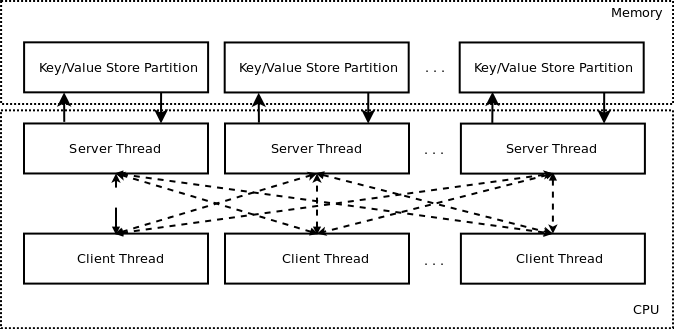
\includegraphics[width=0.8\linewidth]{figs/mcstore.png}
  \caption{\cphash{} Design}
  \label{fig:mcstore}
\end{figure}

  
Section \ref{sec:datastructure} below provides a more detailed description of the partition data structure. 
Sections \ref{sec:serverthreads} \ref{sec:clientthreads} describe the operation of the server and client threads in more detail. 
Section \ref{sec:msgpassing} describes our high performance message passing mechanism that uses buffering and batching. 
In Section \ref{sec:compmigration} we present benefits of computation migration. 

\section{Data Structure}
\label{sec:datastructure}

Every single partition in \cphash{} is a separate hash table. Figure \ref{fig:partition} shows the partition data structure.
Each partition contains a Bucket array. Each Bucket is a linked list. Keys are placed into different buckets based on a hash 
function that maps a key to a specific bucket. Each partition also has an LRU linked list that holds 
elements in the least recently used order. We use LRU list to determine which elements to evict from
a partition when there is not enough space left to insert new elements.

We pre-allocate the space that a partition can use to store data elements at initialization. 
Each element stored consists of a \texttt{key}, a \texttt{pointer} to a value, and a \texttt{size}. 
In \cphash{} the keys are limited to being 60-bit integer numbers; however, this can easily be 
extended to support any key size (see Section \ref{sec:anykey} for more details). 

\begin{figure}[!ht]
  \centering
  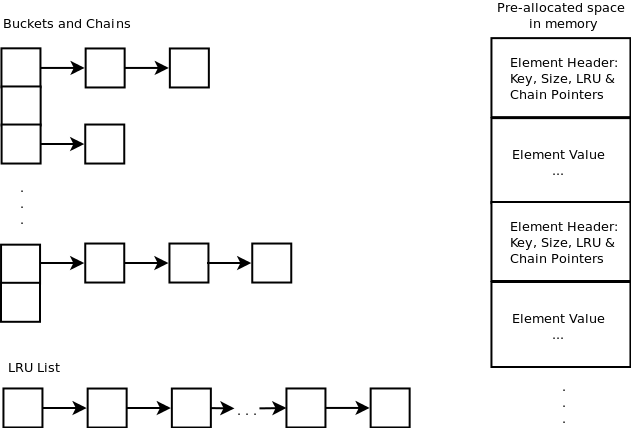
\includegraphics[width=0.8\linewidth]{figs/partition.png}
  \caption{Partition Data Structure}
  \label{fig:partition}
\end{figure}

\section{Server Threads}
\label{sec:serverthreads}

Each server thread is responsible for all the operations that are done on a single partition. 
The server thread continuously loops over the message queues of each client checking for new requests. When requests arrive, the 
server thread performs the requested operation and sends its result back to the client. 

\cphash{} supports two types of operations: \texttt{Lookup} and \texttt{Insert}. 
In the case of a \texttt{Lookup}, the message contains the requested \texttt{key}. If a key/value pair with the given 
\texttt{key} is found in the partition, then the server thread updates the head of the partition's LRU list and return the \texttt{pointer} to the 
value to the client thread; otherwise, the server returns a \texttt{NULL}.

Performing an \texttt{Insert} operation is slightly more complicated. \cphash{} is non-intrusive and 
supports arbitrary length values; thus, every time an insert operation occurs, space must be allocated 
in memory for the value to be copied over. In \cphash{}, the space for the value is allocated by the server 
thread but the data itself is copied by the client thread. Thus, to perform an \texttt{Insert} operation, the server needs 
to receive the \texttt{key} and the \texttt{size} of the data. The server thread allocates \texttt{size} amount of space and removes the existing 
key/value pair with the given \texttt{key} (if it exists) from the partition to avoid having duplicate keys for two different 
elements. The server returns a pointer to the allocated space to the client, which the client later fills in with the
actual data. Chapter 4 goes into more detail on how exactly the memory management works. 
  
\section{Client Threads}
\label{sec:clientthreads}

Applications have client threads that communicate with the server threads to get the queries done. 
Client threads do not necessarily have to be pinned to a specific core but, to achieve the highest performance 
in message passing, it is best to keep the client threads attached to a specific core. An example of a client 
thread in an application would be the client thread in \cpserver{} implementation. The client threads in \cpserver{} 
gather queries from the TCP connections, route them to the appropriate server threads, gather the results, and 
send them back to the correct TCP connections. Chapter \ref{chap:cpserver} describes the \cpserver{} implementation
in more detail.

\section{Buffering and Batching}
\label{sec:msgpassing}

\cphash{} implements message passing between the client and server threads using pre-allocated circular buffers in shared memory. 
For each server and client pair there are two buffers $-$ one for each direction of communication. Another possible way to 
implement message passing could have been to use single value communication. Figure \ref{fig:mpdesign} gives graphical representation for both designs.

In the single value communication pattern, space is allocated for each client/server pair and when a client wants to make 
a request to a server, it modifies this location with its query and waits for the server to respond. When the server is done processing the query it 
updates the shared location with the result. 

The implementation of a single one-way circular buffer consists of the following: a data buffer array, a read index, 
a write index, and a temporary write index. The buffer uses a single producer $-$ single consumer pattern. When the producer wants to add 
data to the buffer, it first makes sure that the read index is large enough compared to the temporary write index so that no 
unread data will be overwritten. Then it writes data to buffer and updates temporary write index. When the temporary write 
index is sufficiently larger than the write index, producer flushes the buffer by changing the write index to the temporary write index. 
To read data, the consumer waits until the read index is less than the write index, then it proceeds to read data and update the read 
index. The Read Index, Write Index and Temporary Write Index are carefully aligned in memory to avoid any false sharing. 
To decrease the number of cache misses when reading or writing buffers, the client threads flush the buffer when the whole cache line is 
full and the server threads update the read index after they are done reading all the queries in a cache line.

\begin{figure}[!ht]
  \centering
  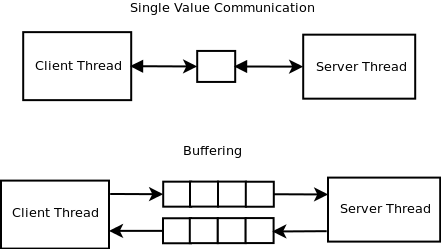
\includegraphics[width=0.8\linewidth]{figs/mpdesign.png}
  \caption{Message Passing Designs}
  \label{fig:mpdesign}
\end{figure}

There are two major benefits to using buffers instead of single value communication. The first advantage is improved parallelism. 
With buffers, the client can just queue the requests to the servers; thus, even if the server is busy, the client can continue working 
and schedule queries for other servers. This way all the servers can stay busy 100\% of the time, thus increasing the overall 
performance. The second reason is the decreased message passing overhead.  With single value communication, for every query 
received, the server would experience a cache miss; however, since the size of the cache line consists of multiple longs (in our test 
machines it is 64 bytes), with buffering the server can receive multiple requests using only a singe cache miss. Figure \ref{fig:mpdesign} 
shows the graphical representation of both designs.

With benefits there are some downsides to using buffers instead of the single value communication pattern. The circular buffer 
implementation requires having extra indices to enable the server and the client to know how much data has been written 
and how much has been read. Maintaining these indices introduces extra performance overhead that single value communication 
does not have. Thus, if the client sends requests to the server at a slow rate, single value communication would 
outperform the buffering implementation. However, if the client has a batch of requests that it needs to complete, buffering will be 
an advantage. Since we are improving the hash table data structure to target applications that are bottlenecked by 
the performance of the hash table, there should be no shortage of requests; therefore, buffering is a better design choice for 
message passing.

\section{Advantages of Computation Migration}
\label{sec:compmigration}

There are several advantages to using computation migration. The first advantage is having a better cache performance 
due to the fact that each partition is only modified and accessed by a single server thread, i.e. a single core. 
Since there is only one core accessing and modifying the data, there are no invalidations for data that 
is written. Furthermore, all frequently accessed structures, such as, the LRU list, buckets array, free list, etc can stay in 
the cache and can be read and modified fast. This provides a significant overall performance increase. 
Chapter \ref{chap:eval} reports on measurements that quantify the performance increase.

The second advantage is being able to get rid of synchronization mechanisms for shared data access and modification. 
Since each partition is modified by only a single core, there is no need for any synchronization mechanisms 
to protect the data from races. In addition to performance benefits, this approach also provides the benefit of ease of 
implementation. With computation migration the actual data structure operations are single threaded and, thus, no 
changes are necessary from the single threaded implementation. 

The more difficult part of the computation migration implementation lies with message passing; however, the message passing design 
and implementation can be standardized and the message passing design and implementation can stay exactly the same for many other data structures. 
Otherwise, to gain good scalability and performance for each specific data structure, different designs for synchronization would be 
necessary. For more complicated data structures the synchronization design can get very complicated with all 
possible cases of race conditions and data paths, thus leading to more potential implementation bugs. 
Computation migration provides an easier way to adopt a previous implementation of a single-threaded data structure 
into a more scalable one.


\section{Memory Management}

To implement a non-intrusive hash table, in addition to storing keys and pointers to the values, the actual value data
needs to be stored. In order to store arbitrary length values, \cphash{} needs the ability to allocate space in memory 
when inserting an element and free it when \cphash{} evicts an element from the hash table. We also need to decide 
which thread (server or client) should be responsible for data allocation and which thread should be responsible 
for copying the data into the allocated space. Freeing values is complicated by the fact that each value can be in use 
in multiple client threads; thus, we need some way of determining when it is actually safe to free and reuse 
the space used by a data value.

Section 4.1 discusses allocation strategies and provides details on our actual implementation. Section 4.2 
discuses strategies for freeing and deallocation. In Section 4.3 we discuss the alternative strategy of reference counting.

\subsection{Allocation}

The best place to do space allocation is in the server thread since each server is responsible for a single partition and 
implementing space allocation would be as simple as implementing a space allocator for a single-threaded hash table. 
However, performing the actual data copying in the server thread would be a bad idea since for large values it would 
wipe-out the local hardware cache of the server core. Thus, in \cphash{} the space allocation is done in the server 
thread and the actual data copying is performed in the client thread. To perform an \texttt{Insert} operation, the client sends the \texttt{key} and 
the \texttt{size} of the value to the server. The server allocates \texttt{size} amount of space in memory and returns 
the pointer to the allocated memory to the client. The allocated space is marked as NOT READY and will not be used until it is marked as READY. 
The client receives the pointer, copies the data to the location pointed by the given pointer, and marks that space as READY. 
The current \cphash{} implementation this marking is done using atomic operations. In Section 4.3 we discuss an alternative 
to it using message passing.

There are many different ways to perform data allocation in the server thread. The simplest way is to use C standard 
\texttt{malloc}/\texttt{free} operations. However, in a heavily multi-threaded environment the libc standard \texttt{malloc} performs poorly. 
A better alternative could be to use memory allocators designed for multi-threaded programs such as streamflow \cite{streamflow}, 
or tcmalloc \cite{tcmalloc} or any other multi-threaded allocator. However, since in \cphash{} the total space is split equally 
between partitions, we decided to just pre-allocate all of the available space for each partition and then use the standard
single-threaded binning allocator \cite{binallocator} inside that pre-allocated space. This way the server threads will never have to communicate when 
allocating or freeing space. 

\subsection{Deallocation/Freeing}

When the server thread evicts or deletes an element from the hash table, the space allocated for this value must to be 
freed so that it can be reused for new elements. It would be incorrect for server thread to just free the allocated space when it evicts or deletes 
the element. The problem is that if a client requests a \texttt{Lookup} on some element X and gets the pointer to its value, 
and then the server threads evicts the element X from the hash table before the client is done processing X's value, the client will have a dangling 
pointer pointing to unallocated space, potentially causing all kinds of errors. To resolve this issue, \cphash{} counts references to the elements. 
Each element in the hash table has a reference count. Every time a client requests a \texttt{Lookup} of an element, the server thread increases the element's 
reference count. When the client is done with the item it decreases the reference count of the given element. When the reference count reaches 0, 
the space can be safely deallocated. We implemented reference counting using atomic operations.

The deallocation must be done by server threads, otherwise there would be race conditions between allocations 
and deallocations for a partition. When a client dereferences an element and its reference count becomes zero we need 
some way to schedule an element for freeing in the server thread. It is worth noting that this is, in general, a highly unlikely 
scenario, especially if clients process elements quickly, since if an element was just accessed in the hash table, it 
would become the most-recently used item thus significantly decreasing chances of its eviction before the client is done processing it.

To implement scheduling of elements for freeing, we implemented a lock-free singly-linked list using atomic operations that holds 
the list of elements that can be safely freed. Scheduled elements are freed in the server thread before the next allocation.

\subsection{Atomic Operations VS Message Passing}

As mentioned in previous sections we implemented the necessary synchronization for memory management using hardware-supported atomic 
operators. Another way to implement reference counting could have been using message passing. Instead of the client thread 
updating the reference count, it would send a message to the appropriate server to update the reference counter. However, in this 
case, message passing is not the best option for several reasons. Since message passing is implemented 
using shared memory and without special hardware support, sending a single message is just as expensive as a single write 
to a memory location. Also in most common cases when a client needs to update the reference count, the counter is already in 
the client's cache thus making those atomic operations fast. The message passing version could become a more viable option 
if the hardware had some special support for fast core-to-core communication.

Another alternative way to implement reference counting would be to send a single message to the server to release all pointers 
per batch. However, that would require the server thread to store all the pointers allocated during the last batch for each client. 
This would impose a significant overhead on the server's local hardware cache, especially if the batches are large. Also it would provide less 
flexibility for a client to decide when to release values.

\section{\cpserver{} Design}
\label{chap:cpserver}

To demonstrate the benefits of \cphash{} in an application we developed, \cpserver{}, a memcached style
Key/Value Cache Server, which uses \cphash{} to implement its hash table.
\cpserver{} has server and client threads as described in Chapter \ref{chap:mcstore}; however,
it also has clients that connect to the server using TCP connections. To avoid confusion with names of client threads and
clients that connect over TCP, we will call the latter TCP clients. Figure \ref{fig:mcserver} shows the design of \cpserver{}.

The server threads operate as described in Chapter \ref{chap:mcstore}. Client threads monitor TCP connections assigned to them 
and gather as many requests as possible to perform them in a single batch. Then, as described in Chapter \ref{chap:mcstore}, client threads pass the 
requests to the appropriate server threads using message passing. After the server threads are done and the client threads receive their results back, they write back 
those results to the appropriate TCP connections. 

The \cpserver{} also has a TCP server thread that accepts new connections. When a connection is made, 
it is assigned to a client thread with the smallest number of current active connections. For our testing needs this simple type of load balancing works fine, 
however the load balancer could be more advanced for work loads in which the traffic on different connections differ significantly.


\begin{figure}[!ht]
  \centering
  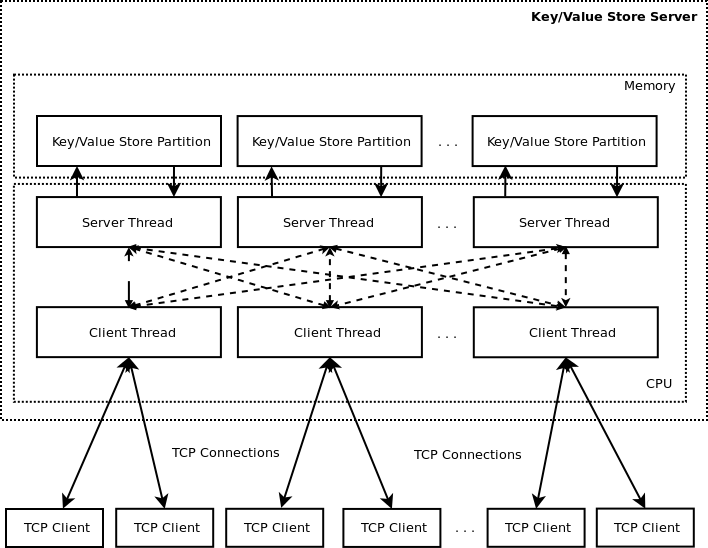
\includegraphics[width=1.0\linewidth]{figs/mcserver.png}
  \caption{\cpserver{} design}
  \label{fig:mcserver}
\end{figure}

\subsection{Protocol}

\cpserver{} uses a simple binary protocol. Figure \ref{fig:protocolrequest} presents binary format of a request header.
Figure \ref{fig:protocolresponse} present binary format of a response.

\begin{figure}[!ht]
  \centering
  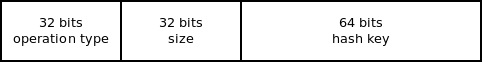
\includegraphics[width=0.8\linewidth]{figs/protocolrequest.png}
  \caption{\cpserver{} request header}
  \label{fig:protocolrequest}
\end{figure}

Two operation types currently supported are: LOOKUP and INSERT.
\begin{description}
\item[LOOKUP] With the LOOKUP request the TCP client asks the server to try to find a key/value pair in the hash table
such that the key matches the \texttt{hash key} field from the request. The \texttt{size} field is unused for the LOOKUP request,
thus it can be set to any value.
\item[INSERT] With the INSERT request the TCP client asks the server to insert a new key/value pair in the hash table. 
The \texttt{hash key} field is the key to be inserted. The \texttt{size} field is the size of the value to be inserted in the hash table.
The INSERT request header is followed by \texttt{size} amount of bytes which describe the value to be inserted.
\end{description}

The actual supported size of the hash key in \cphash{} is 60 bits, thus the most significant 
4 bits of the \texttt{hash key} field will always be ignored by the server.

\begin{figure}[!ht]
  \centering
  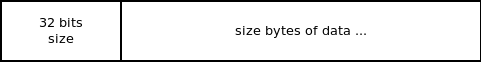
\includegraphics[width=0.8\linewidth]{figs/protocolresponse.png}
  \caption{\cpserver{} response}
  \label{fig:protocolresponse}
\end{figure}

The responses for currently supported operations are the following:
\begin{description}
\item[LOOKUP] For the LOOKUP requests, if a key/value pair is found in the hash table such that the key matches
the \texttt{hash key} provided in the LOOKUP request, then the size of the value and the actual value data are returned.
Otherwise if such a key/value pair can not be found in the hash table, a response with a \texttt{size} of 0 is
returned.
\item[INSERT] The INSERT requests are silent, thus for them there is no response returned from the server.
\end{description}

\subsection{Handling Any Size Keys}
\label{sec:anykey}

In our current implementation only 60 bit hash keys are supported. This can easily be extended to any size keys
without modifying \cpserver{}. The main idea to support any size keys is to use the 60 bit hash of the given any size key as a hash key and store both the 
key and the value together as a value. Then to perform the LOOKUP of a certain key, we would first calculate the hash key
and lookup the value associated with it. If such a value exists it would contain both the key string and the value string in
it. Then before returning the value we would compare the key string to the actual key that we wanted to lookup and if
return the value. If the key strings do not match, this would mean we got hash collision since their hash values match but the 
strings itself do not. In this case we would just return that the value was not found. The chance of collision with 60 bit keys 
would be very small, especially considering the fact that the hash table is stored in memory thus it can not have more than 
couple billion elements in it.

To perform the INSERT operation we would calculate the hash key from the key string and insert a key/value pair in the hash table
where the key would be our calculated hash key and the value would be a combined string of both the key and the value.


\section{Performance Evaluation}
\label{chap:eval}

In this chapter we discuss the performance results that we achieved using \cphash{} and \cpserver{}. In the following sections we 
first discuss our alternative implementations that were developed for comparative benchmarking. Then we present our evaluation of the scalability 
and performance of \cphash{}. Finally we provide the benchmark results for \cpserver{}

\subsection{Alternative Hash Table and Key/Value Cache Server Implementations using Locks}

To evaluate the performance and scalability of \cphash{}, we created an alternative implementation
of the hash table that does not use computation migration. This version is implemented in a traditional shared memory 
style with scalable fine-grained locks. In this alternative implementation, each partition is protected by
a lock and there are no server threads. The client threads process queries by first acquiring the lock for
the appropriate partition, then performing the query, updating the LRU list and, finally, releasing the lock. We call this implementation \lockhash{}.
We use this alternative implementation for comparison with \cphash{} to show that computation migration provides much
better scalability and performance than having scalable locks.

In addition to developing the alternative hash table implementation we also developed an alternative key/value cache server implementation
that uses \lockhash{} as its hash table instead of \cphash{}. We call this alternative server implementation \lockserver{}.

\subsection{Hash Table Performance}

We created a simple benchmark that tests various aspects of the hash table implementations. The benchmark generates random queries and
performs them on the hash table. A single query can be either a LOOKUP or an INSERT operation. The INSERT operation consists of 
inserting key/value pairs such that the key is a random number and the value is the same as the key (8 bytes). 

The benchmark can be configured using several parameters:
\begin{itemize}
\item Number of Partitions (i.e. number of server threads)
\item Number of Client Threads/Cores
\item Size of Batch
\item Maximum cache size in bytes
\item Hash INSERT ratio over total number of queries
\item Maximum Value of Hash Key
\item Number of iterations
\end{itemize}

We use a 48 core AMD64 machine for our testing. This machine has eight six-core processors of type AMD Opteron(tm) 8431. Each core has
a 512KB L2 cache and each six-core processor has a unified 6MB L3 cache.

\subsubsection{Scalability}

The first experiment evaluated the scalability of the \cphash{} implementation. We ran our benchmark with an equal number of server 
and client threads varying from 3 to 24 (i.e. using 6 to 48 cores $-$ half of the cores for the server threads, and the other half for the 
client threads), with a total hash table size of 10 MB, with 30\% INSERT ratio, with keys ranging from 0..$2^{17}$, and for $10^{8}$ iterations. 
We also ran our \lockhash{} implementation with the same exact parameters using 6 to 48 cores. Figure \ref{fig:scale10mb} shows the 
throughput per core for \cphash{} and \lockhash{} on a 10 MB hash table.

We also ran the same tests but with a hash table size of 1 GB with keys ranging from 0..$2^{24}$. In this case, we ran the benchmark for $10^{9}$ iterations to make
sure that the hash table was full for most of the iterations. Figure \ref{fig:scale1gb} shows the throughput per core for \cphash{} and \lockhash{} on the
1 GB hash table.

\begin{figure}[!ht]
  \centering
  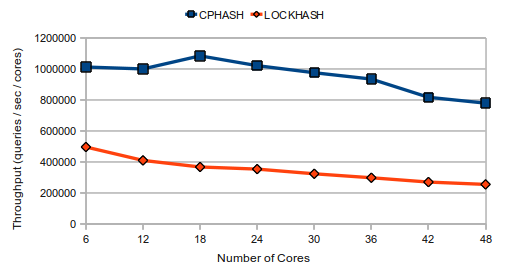
\includegraphics[width=0.8\linewidth]{figs/scale10mb.png}
  \caption{Throughput per core on 10 MB hash table}
  \label{fig:scale10mb}
\end{figure}
    
\begin{figure}[!ht]
  \centering
  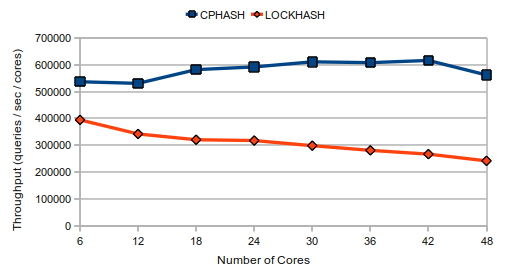
\includegraphics[width=0.8\linewidth]{figs/scale1gb.png}
  \caption{Throughput per core on 1 GB hash table}
  \label{fig:scale1gb}
\end{figure}

These graphs show that the \cphash{} implementation has better scalability than the \lockhash{} implementation. However, we do not 
get a complete linear speedup for small hash tables. The reason for this is the message passing overhead. This overhead is more significant for smaller 
hash tables since most other memory operations are cache hits, thus, message passing takes a significant percentage of the total computation time. On
the other hand \cphash{} achieves great scalability for larger hash table. It achieves a super-linear speedup in Figure \ref{fig:scale1gb} due to the fact that
as the number of cores increases, its combined L2 and L3 cache space is larger, resulting in fewer cache misses per query and higher throughput per core. 

As the number of cores increases, message passing becomes more expensive due to the hardware architecture. If the cores are physically farther apart from each 
other, the message passing cache miss will take longer to complete. To prove this hypothesis we ran our benchmark with a small empty hash table, and no INSERTs. 
In this scenario message passing takes most of the computation time. Figure \ref{fig:scalemp} shows the declining throughput as the number of cores increases.

\begin{figure}[!ht]
  \centering
  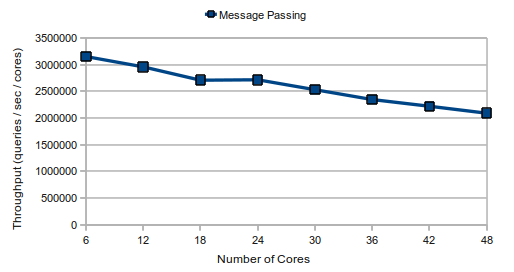
\includegraphics[width=0.8\linewidth]{figs/scalemp.png}
  \caption{Message Passing Throughput per core}
  \label{fig:scalemp}
\end{figure}

\subsubsection{Performance}

Figure \ref{fig:cphashspeedup} shows the throughput gains of \cphash{} compared to the \lockhash{} implementation for the tests described in 
the previous section, as well as for a 40 MB hash table.

\begin{figure}[!ht]
  \centering
  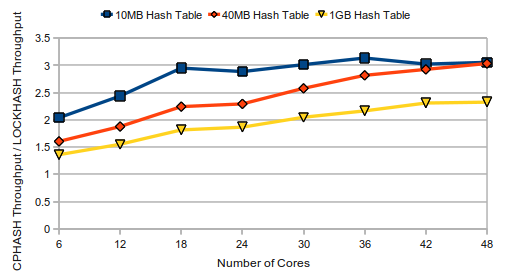
\includegraphics[width=0.8\linewidth]{figs/cphashspeedup.png}
  \caption{\cphash{} throughput vs \lockhash{} throughput}
  \label{fig:cphashspeedup}
\end{figure}

The performance of \cphash{} does not depend on the actual size of the hash table but rather on the number of elements in it. This is because the server 
threads never access or modify the values in the hash table but just the meta data (buckets, chain lists, LRU list etc). In our benchmarks the value of 
each element has the same size (8 bytes), therefore, the number of elements in the hash table is proportional to the size of the table.

The results shown in Figure \ref{fig:cphashspeedup} are consistent with the scalability graphs. \cphash{}'s throughput per core decreases after all 
the hash table meta data fits in the combined hardware caches of the server cores. This is the main reason why we do not see any increase in throughput ratio after 
the number of cores reaches 18, for 10 MB hash table. The current bottleneck for scalability on small hash tables is the \cphash{}'s message passing implementation.

\subsubsection{Summary}

The benchmark results show that \cphash{} is scalable and provides increased throughput, especially when the hash table meta data fits in the server cores'
combined hardware caches. When the hash table meta data is much larger than the combined caches, \cphash{} still provides some benefits through batching and caching 
the common partition data (such as an LRU list).

There is another scenario when \cphash{} is beneficial for large hash tables. Even though most of the time the load on the hash table may not be significant
and the performance is acceptable, there might be certain peak times when a specific small subset of the hash table experiences heavy load (i.e. most of the queries involve 
operations on keys in that subset). If this subset is small enough so that its meta data fits into the combined caches of server cores, then the \cphash{} 
implementation can significantly improve performance.

\subsection{Key/Value Cache Server Performance}
\label{sec:mcserverbench} 

We tested the performance of our \cpserver{} against the \lockserver{} and \memcached{}. For these benchmarks we used a 16 core AMD64 machine as 
our server. This 16 core machine has four quad-core processors of type AMD Opteron(tm) 8350. Each core has a 512KB L2 cache, and each quad-core processor has a 
unified 4MB L3 cache. 

We developed a benchmark client for the Key/Value Cache Server. We used our 48 core AMD64 machine as a load generator to run the benchmark clients. 
The load generator machine and the server machine were connected with 10 GBit Ethernet network. We made sure in our benchmarks that we were generating enough load to 
bottleneck the servers, so that the speed of a single benchmark client would not affect the performance. We also made sure that the servers were CPU and Memory 
bottlenecked and that the network was not the limiting factor. To achieve this, in addition to having 10GBit Ethernet network, we used a 
patch for the Linux kernel network driver \cite{mosbench} to make it more scalable.

The benchmark client has following configuration parameters:
\begin{itemize}
\item Size of Batch
\item Hash INSERT ratio over total number of queries
\item Maximum Value of Hash Key
\item Size range for Hash Value
\item Number of iterations
\end{itemize}

First we compared the performance of \cpserver{} to \lockserver{}. We ran the servers with a 16 GB hash table. Before starting any benchmarking we 
made sure to completely fill up the hash table with random data. We set the batch size to 1000, and the size range for the hash values to 8$-$128 bytes. We run our tests 
for 80 million iterations.

We varied the INSERT ratio from 0\% to 100\% with 20\% steps. We tried three different Hash Key ranges: 0..2$^{16}$, 0..2$^{23}$, and 0..2$^{28}$. A 16 GB hash table
can hold around 160 million elements when the size of values are 8 to 128 bytes. Therefore when running with Hash Key ranges of 0..2$^{16}$ or 0..2$^{23}$, the hit rate 
is 100\%. On the other hand when running with a key range of 0..2$^{28}$ it is around 60\%-70\%. Figure \ref{fig:cpserverspeedup} shows the throughput gains of 
\cpserver{} compared to \lockserver{}.

\begin{figure}[!ht]
  \centering
  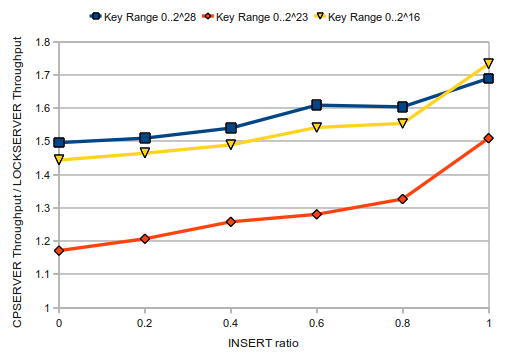
\includegraphics[width=0.8\linewidth]{figs/cpserverspeedup.png}
  \caption{\cpserver{} throughput vs \lockserver{} throughput}
  \label{fig:cpserverspeedup}
\end{figure}

There are four major factors that affect the speedup: Hit Rate, INSERT ratio, size of the hash table (or the range of hash keys), and the size of the hash values. 
Smaller Hit Rate and higher INSERT ratio result in larger speedups for \cpserver{}. This is because hash INSERTs are silent (i.e. the server does not return 
any response for them), and LOOKUP misses just return a single 32 bit value. Thus, for hash INSERTs and LOOKUP misses, most of the computation time for a query is taken by 
the hash table operation and not by the writes to the TCP connection buffer. 

Larger hash values work against the \cpserver{} implementation. If hash values are large most of the computation time during LOOKUP query hits is spent on 
writing back the value to the TCP buffer. For very large hash values the \lockserver{} can outperform the \cpserver{} since it has more threads 
writing to the buffers which results in better performance.

The size of the hash table or the range of the hash keys affects performance since, as we showed in the previous section, if the meta data of all the elements 
that are accessed can fit into the combined caches of the server cores, the hash operations in \cphash{} will be faster than in \lockhash{}.

Figure \ref{fig:cpserverspeedup} confirms our hypotheses. With key ranges of 0..2$^{16}$ or 0..2$^{23}$ the hit rate is 100\%; however, the meta data of 
2$^{16}$ elements fits into the combined caches of 8 server cores, resulting in a higher speedup. For the key range of 0..2$^{28}$ the hit rate is around 65\%; 
therefore, there is less time spent on writing buffers and more time spent on the actual hash operations resulting in a higher overall speedup.

\subsubsection{Performance against \memcached{}}
We compared the performance of \cpserver{} to \memcached{}. We ran 16 \memcached{} servers with 1 GB size limit each (16 GB total) on our server machine.
We extended the benchmark client with the \texttt{libmemcached} library \cite{libmemcached} to run same the benchmarks for \memcached{} as the ones described in
the previous section. However, since the \memcached{} protocol supports batching only for LOOKUPs, we performed the tests with only LOOKUP operations. As in previous 
test runs we made sure to fill up hash table server with some random elements before running any benchmarks. 

We ran tests with two different hash value size ranges: 8 to 128 bytes and 8 to 512 bytes. 
Tables \ref{table:memcachedspeedup0} and \ref{table:memcachedspeedup1}, show the results for the two scenarios described.

Since the \memcached{} protocol has a higher overhead per each request and response sent, we also compared the performance of \cpserver{} with hash value 
ranges of 72 to 192 bytes to \memcached{} with value ranges of 8 to 128 bytes. The results for this test run are provided in Table \ref{table:memcachedspeedup2}.

The tables give total running times for \cpserver{} and \memcached{} (in seconds) and also provide the average hit rate per each LOOKUP operation.
Figure \ref{fig:cpserverspeedup2} shows the throughput gains of \cpserver{} compared to \memcached{} based on values provided in the tables. 

\begin{table}[!ht]
\centering
\caption{Speedup with hash value size range of 8 to 128 bytes} 
\label{table:memcachedspeedup0}
\begin{tabular}{ | c | c | c | c | c | }
  \hline
  Key Range & \cpserver{} & \memcached{} & Speedup & Hit rates \\
  \hline
  0..2$^{28}$ & 13.563 & 35.618 & 2.626 & 0.655 vs 0.817 \\
  0..2$^{23}$ & 22.102 & 39.741 & 1.798 & 1.0 vs 1.0     \\
  0..2$^{16}$ & 16.719 & 39.512 & 2.363 & 1.0 vs 1.0     \\
  \hline
\end{tabular}
\end{table}

\begin{table}[!ht]
\centering
\caption{Speedup with hash value size range of 8 to 512 bytes} 
\label{table:memcachedspeedup1}
\begin{tabular}{ | c | c | c | c | c | }
  \hline
  Key Range & \cpserver{} & \memcached{} & Speedup & Hit rates \\
  \hline
  0..2$^{28}$ & 27.587 & 41.753 & 1.514 & 0.688 vs 0.750 \\
  0..2$^{23}$ & 43.532 & 46.251 & 1.062 & 1.0 vs 1.0     \\
  0..2$^{16}$ & 39.845 & 46.388 & 1.164 & 1.0 vs 1.0     \\
  \hline
\end{tabular}
\end{table}

\begin{table}[!ht]
\centering
\caption{Speedup with larger hash value size range for \cpserver{}} 
\label{table:memcachedspeedup2}
\begin{tabular}{ | c | c | c | c | c | }
  \hline
  Key Range & \cpserver{} & \memcached{} & Speedup & Hit rates \\
  \hline
  0..2$^{23}$ & 23.240 & 39.741 & 1.710 & 1.0 vs 1.0   \\
  0..2$^{16}$ & 19.329 & 39.512 & 2.044 & 1.0 vs 1.0   \\
  \hline
\end{tabular}
\end{table}

\begin{figure}[!ht]
  \centering
  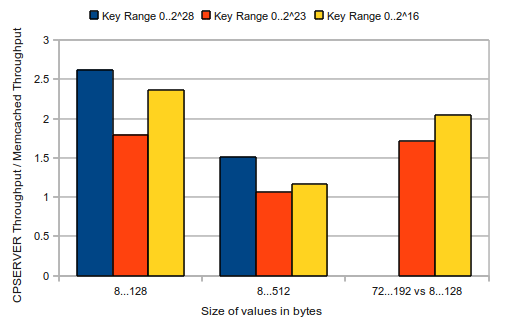
\includegraphics[width=0.8\linewidth]{figs/cpserverspeedup2.png}
  \caption{\cpserver{} throughput vs \memcached{} throughput}
  \label{fig:cpserverspeedup2}
\end{figure}

The results achieved are similar to the results achieved against \lockserver{}. Smaller hit rate, smaller values and smaller key range all benefit the
\cpserver{} implementation for the same reasons as described in the previous section. On the other hand, as can be noticed in the second row of Table 
\ref{table:memcachedspeedup1}, when the hit rate is 100\% and the value range is 8 to 512 bytes, \cpserver{} has almost no advantage over \memcached{},
especially when the size of hash table is much larger than size of combined L2 and L3 caches of all the server cores.

The results indicate that \cpserver{} outperforms \memcached{} in several specific scenarios; however, a performance evaluation with a load specific to a 
real-world application or web-server is needed for a more comprehensive comparison of the two server implementations. 


\chapter{Future Work}
\label{chap:futurework}

\cphash{} demonstrates that by using computation migration, message passing and careful memory management techniques it is
possible to create a scalable hash table implementation for the multi-core NUMA architecture machines. However, there is still
room for improvement of \cphash{}'s implementation. 

\section{Dynamic Adjusting of the Server Threads}

One issue with the current design is that a fixed number of cores must to be dedicated to run the server threads. 
A better approach would be to have an algorithm that would dynamically decide on how many cores to use for the server threads, 
depending on the workload. Such dynamic adjustment of the server threads would make it possible to use less power and CPU resources
when the workload is small. Saving power is essential for any data center due to reduced cost. Using less CPU resources
would make it possible to run other services on the same machine when there is not much load on the hash table. 

Dynamic adjustment of the server threads could also provide higher performance. 
If the CPU resources needed by the client threads to generate the queries is less than the resources needed by the server threads 
to complete the queries, then it is better to dedicate more cores to run the server threads than to the client threads. 
On the other hand, if the client threads need more CPU resources to generate the queries, it is better to dedicate fewer cores to run
the server threads and use more cores for the client threads. 

We have not tried implementing dynamic adjustment of server threads due to time constraint reasons; however, we tried
a different approach to avoid wasting the CPU resources. We tried utilizing CPUs with Intel's HyperThreading technology to run 
the server and the client threads on two separate logical cores of the same physical core. The problem we discovered with this approach is that 
since the logical cores share the L2 cache, the client thread can easily pollute the whole cache thus nullifying most of the benefits of the \cphash{}
design. This is especially true for an application such as \cpserver{}, since the connection buffers themselves can take most of the space in the cache.

\section{Message Passing}

The scalability and performance of message passing is important for \cphash{}. The current implementation is simple and does not use
any hardware specific operations to further speedup the communication between the server and the client threads. One possible improvement is to
forcefully flush the caches when the buffer is full, this way the overhead of sending the message would shift more from the receiver towards the sender. 
Such an approach could be beneficial to decrease the time spent on reading the message buffers in server threads. Such an approach could potential provide
more scalable message passing implementation. 

Another idea to improve the current message passing implementation is to change the design of the circular buffer to eliminate the read and write indexes
to further decrease average cache misses spent on message passing per each query. 


\section{Conclusion}

In this thesis we introduced \cphash{} $-$ a scalable fixed size hash table implementation that supports eviction
using an LRU list, and \cpserver{} $-$ a scalable in memory key/value cache server implementation that uses \cphash{}
as its hash table. 
Experiments on a 48 core machine showed that on a small hash table \cphash{} has 3 times higher throughput than a hash
table implemented using scalable fine-grained locks. On a large hash table \cphash{} had 2 times higher throughput than
a hash table implemented using scalable locks. 
\cpserver{} achieved 1.2 to 1.7 times higher throughput than a key/value cache server 
that uses a hash table with scalable fine-grained locks, and 1.5 to 2.6 times higher throughput than \memcached{}.

The improved performance is due to the reduced number of cache misses per operation. The number of cache coherency misses
is reduced due to caching common partition data that are modified, which in \cphash{} is the head of the LRU list. 
For small hash tables, the number of cache capacity misses is reduced, since \cphash{} avoids the data duplication in local hardware
caches by transferring the computation between the cores instead of the data.


\appendix
\bibliographystyle{abbrvnat}
\bibliography{main}

\end{document}

